\section{Introduction \& Motivating Example}
One of the first steps in designing a new Domain-Specific Language (DSL) is to choose which \emph{language vehicle} (LV) will be used to engineer it.
We define a LV as the technological means for implementing a language.
This includes language workbenches as well as programming languages and ontology languages, to name a few.
%A language vehicle may pertain to any \emph{technological space} (TS) such as grammarware, modelware, PLware, \etc.
The notion of language vehicle is orthogonal to the distinction between technological spaces (\eg~grammarware, modelware~\cite{kurtev2002technological}); between graphical and textual syntax; between internal, embedded, and external DSLs,~\etc.
%\footnote{In this paper, we build upon \citeauthor{kurtev2002technological}'s view of a TS:~``a working context with a set of associated concepts, body of knowledge, tools, required skills, and possibilities''~\cite{kurtev2002technological}.}
%In addition, we consider a cohesive set of tools in a given TS (\eg~a particular language workbench) as a separate TS.
For instance, we consider Rascal~\cite{klint2010easy} and Spoofax~\cite{kats2010spoofax} as two distinct language vehicles within the broader technological space of grammarware and meta-programming; EMF~\cite{steinberg2008emf} and UML~\cite{fowler2004uml} (using Profiles~\cite{selic2007systematic}) as two distinct language vehicles within the broader technological space of modelware.
LVs usually come with their own meta-languages for expressing the various aspects of a DSL:~abstract syntax, concrete syntax, static and execution semantics, tools, \etc.
%Examples of prominent LV include meta-modeling environments such as EMF~\cite{steinberg2008emf}, meta-programming environments such as Rascal~\cite{klint2010easy} and Spoofax~\cite{kats2010spoofax}, projectional environments such as MPS~\cite{voelter2013language}, plain old programming languages such as Racket~\cite{felleisen2018programmable} or Scala~\cite{hofer2010modular}, and language workbenches (LWBs) in general~\cite{erdweg2015evaluating}.
%\td{Sentence above could be shortened/removed}
As implementation techniques radically differ from one LV to another, this initial design choice commits the development of a DSL in a set direction that can hardly be reconsidered later.

From the language designer's point of view, however, every LV has its own strengths.
The ecosystem around EMF excels in the definition of user-friendly editors and persistence frameworks for large models, while the Rascal environment excels in the definition of interpreters and refactoring tools.
%On the other hand, the flexibility of manipulating the concepts of a DSL through a fluent API, using the capabilities of a general-purpose programming language, is unmatched.
The benefits of various LVs are also visible from the language users' point of view.
While domain experts may prefer to manipulate domain concepts through a dedicated syntax, advanced users (\eg~system integrators) may favor the flexibility of a fluent API in their favorite programming language to manipulate the very same constructs.
%However, it is currently not possible to \emph{combine the strengths of multiple LV to engineer a single DSL}.
%\td{Why?}

Let us consider a simple finite-state machine (FSM) language as a motivating example.
As depicted in \Cref{fig:motivating-fsm}, one would like to combine the strengths of multiple LVs to engineer this DSL.
Rascal could be used to develop its interpreter, a set of refactoring tools (\eg~state collapsing and minimization), and a textual editor; EMF to develop a graphical animator for debugging FSM models and a persistence layer; Java to offer a fluent API for advanced users who focus on its integration with other system concerns.

\begin{figure}[bt]
	\centering
	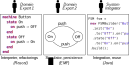
\includegraphics[width=\columnwidth]{figures/motivating-fsm-simplified-2}
	\caption{Three incarnations of the same FSM model in three language vehicles:~different representations and tools for different users and tasks.}
	\label{fig:motivating-fsm}
\end{figure}

Using today's techniques, it is possible to define the same FSM language in these three LVs separately.
It is not possible, however, to apply the tools of a given LV on the models or programs created in another LV---for instance, animating a FSM model written in EMF using the Rascal interpreter, or synchronizing a textual FSM model in Rascal with its equivalent incarnation as a Java AST.
Achieving this goal requires to \emph{efficiently synchronize the diverse representations of the same model in different LVs}; for instance to let the FSM interpreter written in Rascal update its own representation of an FSM model after each execution step and synchronize it with the representation of the same model in EMF for animation purposes.

In this paper, we envision a language engineering approach enabling (i) language designers to combine tools from multiple LVs to engineer diverse shapes for a single DSL and (ii) language users to manipulate language constructs in the most appropriate shape.
%We endeavor to show \emph{how to break down the barriers between different vehicles so that language designers can combine the strengths of each in the engineering of a single DSL, and language users can synchronize their models across various shapes}.
%\emph{Metamorphic synchronization} refers to the possibility of synchronizing different incarnations of the same model in different shapes of a language, \ie~in different vehicles.
%As different vehicles rely on radically different theories, a successful approach for bridging them must thus \emph{align} \td{!no!} them in some way.
We present the notion of shape-diverse DSL in greater depth in \Cref{sec:shapes}.
We then present our prototype approach, \prism, in \Cref{sec:prism}, and discuss our implementation of a shape-diverse FSM language in \Cref{sec:eval}.
Finally, we discuss open questions and possible next steps in \Cref{sec:discussion}.
